\include{lam-ott}
\include{CHSTLC-ott}
\include{CSTLC-ott}
\include{combinatory_logic-ott}
\include{T-ott}
\include{F-ott}
\include{SSF-ott}
\include{Fw-ott}
\include{lamu-ott}
\include{lamd-ott}
\include{lam-bar-mu-mu-tilde-ott}
\include{dual-calculus-ott}
\include{type-theory-ott}
\include{CoC-ott}
\include{CoC_sep-ott}

% Theorems
\newcounter{thm}
%% Resets the thm counter at the start of each section.
\makeatletter
\@addtoreset{thm}{section}
\makeatother
%% This makes sure \ref has the section, subsection, and thm number.
\def\thethm{\thesubsection.\arabic{thm}}
%% This makes the figure numbering match the other environments.
% \renewcommand{\thefigure}{\thesubsection.\arabic{figure}}

\newenvironment{thm}{
 \refstepcounter{thm} \par \addvspace{\baselineskip} \noindent \textbf{\underline{Theorem \thethm.}} \begin{em}
   \begin{changemargin}{1px}{2px}\noindent
}{
  \end{changemargin}
  \end{em} \par \addvspace{\baselineskip} 
}
\newenvironment{lemma}{
  \refstepcounter{thm} \par \addvspace{\baselineskip} \noindent \textbf{\underline{Lemma \thethm.}} \begin{em}
    \begin{changemargin}{1px}{2px}\noindent
}{
  \end{changemargin}
  \end{em} \par \addvspace{\baselineskip}
}
\newenvironment{lemmaItem}{
  \refstepcounter{thm} \par \addvspace{\baselineskip} \noindent \textbf{\underline{Lemma \thethm.}} \begin{em}
}{
  \end{em} \par \addvspace{\baselineskip}
}
\newenvironment{proposition}{
  \refstepcounter{thm} \par \addvspace{\baselineskip} \noindent \textbf{\underline{Proposition \thethm.}} \begin{em}
    \begin{changemargin}{1px}{2px}\noindent
}{
    \end{changemargin}
  \end{em} \par \addvspace{\baselineskip}
}
\newenvironment{corollary}{
  \refstepcounter{thm} \par \addvspace{\baselineskip} \noindent \textbf{\underline{Corollary \thethm.}} \begin{em}
  \begin{changemargin}{1px}{2px}\noindent
}{
  \end{changemargin}
  \end{em} \par \addvspace{\baselineskip}
}
\newenvironment{definition}{
  \refstepcounter{thm} \par \addvspace{\baselineskip} \noindent \textbf{\underline{Definition \thethm.}} 
  \begin{em}\begin{changemargin}{1px}{2px}\noindent
}{
\end{changemargin}
  \end{em} \par \addvspace{\baselineskip} 
}
\newenvironment{example}{
  \refstepcounter{thm} \par \addvspace{\baselineskip} \noindent
  \textbf{\underline{Example \thethm.}} \begin{em}
    \begin{changemargin}{1px}{2px}\noindent
}{
  \end{changemargin}
  \end{em} \par \addvspace{\baselineskip}
}

% Commands that are useful for writing about type theory and programming language design.
\newcommand{\case}[4]{\text{case}\ #1\ \text{of}\ #2\text{.}#3\text{,}#2\text{.}#4}
\newcommand{\interp}[1]{[\negthinspace[#1]\negthinspace]}
\newcommand{\normto}[0]{\rightsquigarrow^{!}}
\newcommand{\join}[0]{\downarrow}
\newcommand{\redto}[0]{\rightsquigarrow}
\newcommand{\nat}[0]{\mathbb{N}}
\newcommand{\terms}[0]{\mathcal{T}}
\newcommand{\fun}[2]{\lambda #1.#2}
\newcommand{\CRI}[0]{\text{CR-Norm}}
\newcommand{\CRII}[0]{\text{CR-Pres}}
\newcommand{\CRIII}[0]{\text{CR-Prog}}
\newcommand{\subexp}[0]{\sqsubseteq}
\newcommand{\napprox}[2]{\lfloor #1 \rfloor_{#2}}
\newcommand{\interpset}{\mathcal{I}}
\newcommand{\powerset}[1]{\mathcal{P}(#1)}
\newcommand{\vinterp}[1]{\mathcal{V}[\negthinspace[#1]\negthinspace]}
\newcommand{\vbinterp}[2]{\bar{\mathcal{V}}_{#1}[\negthinspace[#2]\negthinspace]}
\newcommand{\ginterp}[1]{\mathcal{G}[\negthinspace[#1]\negthinspace]}
\newcommand{\dinterp}[1]{\mathcal{D}[\negthinspace[#1]\negthinspace]}
\newcommand{\tinterp}[1]{\mathcal{T}[\negthinspace[#1]\negthinspace]}


%% Formatting the Ott names.  This is really a bug in Ott.
\renewcommand{\CSTLCdrulename}[1]{\scriptsize \textsc{#1}}
\renewcommand{\CHSTLCdrulename}[1]{\scriptsize \textsc{#1}}
\renewcommand{\CSTLCdrulename}[1]{\scriptsize \textsc{#1}}
\renewcommand{\CoCdrulename}[1]{\scriptsize \textsc{#1}}
\renewcommand{\CoCSdrulename}[1]{\scriptsize \textsc{#1}}
\renewcommand{\Fdrulename}[1]{\scriptsize \textsc{#1}}
\renewcommand{\Fwdrulename}[1]{\scriptsize \textsc{#1}}
\renewcommand{\SSFdrulename}[1]{\scriptsize \textsc{#1}}
\renewcommand{\Tdrulename}[1]{\scriptsize \textsc{#1}}
\renewcommand{\Combdrulename}[1]{\scriptsize \textsc{#1}}
\renewcommand{\DCdrulename}[1]{\scriptsize \textsc{#1}}
\renewcommand{\LBMMTdrulename}[1]{\scriptsize \textsc{#1}}
\renewcommand{\Lamdrulename}[1]{\scriptsize \textsc{#1}}
\renewcommand{\Lamddrulename}[1]{\scriptsize \textsc{#1}}
\renewcommand{\Lamudrulename}[1]{ {\scriptsize \textsc{#1}} }
\renewcommand{\TTdrulename}[1]{\scriptsize \textsc{#1}}

\chapter{A Brief History of Type Theory}
\label{chap:the_history_of_type_theory}
\input{history-inc}
% section the_history_of_type_theory (end)

\chapter{The Computational Trinity}
\label{chap:the_three_perspectives}
The Merriam-Webster dictionary defines ``computation'' as ``the act or
action of computing : calculation'', ``the use or operation of a
computer'', ``system of reckoning'', or ``an amount computed''.  These
meanings suggest computation is nothing more than the process of
mathematical calculation, but computation is so much more than this.
In fact there are three perspectives of computation:
\begin{center}
  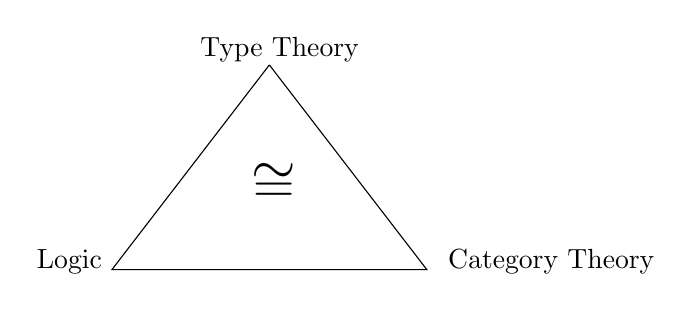
\begin{tikzpicture}       
    \node at (-1.87,3.1) {\text{Type Theory}};
    \node at (-4.54,0.4) {\text{Logic}};
    \node at (1.58,0.4) {\text{Category Theory}};
    \node at (-1.94,1.4) {\huge $\cong$};
    
    %% The left most triangle.
    \draw (-2,2.9) -- (-4, 0.3) -- (0,0.3) -- (-2,2.9);
  \end{tikzpicture}    
\end{center}
Each offering a unique position for studying computational structure.
The figure above illustrates that type theory, category theory, and
logic are equals where the symbol in the middle can be read as
``isomorphic to.''  That is all three fields look very different, but
can be treated as equivalent.  Type theories -- as we have seen above
-- or typed $\lambda$-calculi are essentially the study of functions
where types enforce some properties on these functions.  Now as it
turns out category theory is basically the abstract study of
mathematical structures using the abstraction of a function called a
morphism.  Hence, in hindsight it is not surprising that type theory
and category theory are equals each offering a unique perspective of
computation.  Less intuitive is the connection between these two
fields and that of logic.  Calling this beautiful relationship the
computational trinity is non-standard.  In fact I am proposing that
this terminology become standard.  The standard names for this
relationship is the Curry-Howard correspondence (or isomorphism) or
the proofs-as-programs propositions-as-types correspondence.  The
first pays tribute to Haskell Curry and William Howard. As we will see
both Curry and Howard did have a hand in making this ternary
relationship explicit, but they were not the only ones.  Hence, this
former name is unsatisfactory. The second only signifies the
connection between logic and type theory; it does not mention category
theory.  Thus, it is unsatisfactory.  Therefore, a better name for
this relationship must become standard and I propose the computational
trinity.  Robert Harper calls this connection the ``Holy Trinity'' and
the three way connection given above computational trinitarianism, but
we have chosen to not use religious metafors in computational research.
Thus, we propose the name ``computational trinity'' to emphasize the
common structure between each point, and the fact that it is a three
way connection.  We now move onto making this relationship more
precise.  We only discuss the details of the correspondence of type
theory and logic, and type theory and category theory.  The other
correspondence between logic and category theory follows
similarly. Furthermore, we do not go into complete detail of each of
these correspondences, but we give plenty of references for the
curious reader.

\section{Type Theory and Logic}
\label{sec:type_theory_logic}
Intuitionism began with Luitzen Brouwer.  Implicit in his work was an
interpretation of the formulas of propositional and predicate
intuitionistic logic as computational objects.  Brouwer's student
Arend Heyting made this interpretation explicit for intuitionistic
predicate logic against the advice of Brouwer.  Brouwer believed that
intuitionistic logic should never be written down, but only exist in
the mind of the mathematician.  Additionally, Andrey Kolmogorov
defined this interpretation for intuitionistic propositional logic.
This interpretation has become known as the
Brouwer-Heyting-Kolmogorov-interpretation or the BHK-interpretation of
intuitionistic logic.  Let's consider this interpretation for
intuitionistic propositional logic with conjunction, disjunction, and
implication.  We denote arbitrary computational constructions as $c$
which can be built up from pairs of proof terms $(t_0,t_1)$, unary
functions denoted by $\lambda$-abstractions, and injections for proof
terms for sums $inl(t)$ for inject left and $inr(t)$ for inject right.
The BHK-interpretation defined in Def.~\ref{def:bhk-interpretation}
defines the assignment of proof terms using these constructs to
formulas of intuitionistic propositional logic.

\begin{definition}
  \label{def:bhk-interpretation}
  The BHK-interpretation:\\
  \begin{center}
          \begin{tabular}{lll}
      $c\,r\,(A_1 \land A_2)$ & $\iff$ & $c = (t_0,t_1)$ such that $t_0\,r\,A_1$ and 
            $t_1\,r\,A_2$.\\
      $c\,r\,(A_1 \lor A_2)$  & $\iff$ & ($c = inl(t)$ and $t\,r\,A_1$) or ($c = inr(t)$ and 
            $t\,r\,A_2$).\\
      $c\,r\,(A_1 \to A_2)$   & $\iff$ & $c$ is a function, $\lambda x.t$, such that for any 
            $d\,r\,A_1$ \\
                              &     & $(\lambda x.t)d\,r\,A_2$.
    \end{tabular}
  \end{center}
  We say a construction $c$ realizes $A$ $\iff$ $c\,r\,A$.  
\end{definition}
This was the first step towards the correspondence between type theory
and logic.  The second was due to Curry.  We mentioned in
Section~\ref{chap:the_history_of_type_theory} that Curry noticed that the
types of the combinatory logic correspond to the formulas of
intuitionistic propositional logic.  This suggested that combinatory
logic can be seen as a proof assignment to propositional logic.  This
was Curry's main contribution to this line of work.  The third step
was due to Howard.  In \cite{Howard:1980} Howard revealed the
correspondence between STLC and intuitionistic propositional logic in
natural deduction style.  He essentially uses the BHK-interpretation
to assign proof terms to natural deduction and then shows that this
really is STLC.  It is a beautiful result.  More on this can be found
in
\cite{Griffin:1990,Howard:1980,Mints:2000,Murthy:1991,Sorensen:2006,Troelstra:1991}.
Since these early steps the correspondence between logic and type
theory has been developed quite extensively.  Reynolds' and Girard
extended this correspondence to second order predicate logic using
system F, and to higher order logic using system $\text{F}^\omega$ by
Girard \cite{Wadler:2007,Girard:1971}.  We will see other advances to this
correspondence with logic in Section~\ref{chap:dependent_type_theory} where
we discuss dependent types.

There is one requirement a type theory must meet in order for it to
correspond to a consistent logic. Computational constructs such as
objects of type theory must be total (terminating).  That is they must
always produce a result.  One part of the correspondence between type
theory and logic is that the reduction rules of the type theory amount
to the cut-elimination algorithm for the logic.  That is, reducing
terms amounts to normalizing proofs.  The validity of the cut theorem
-- states that any non-cut-free proof can always be reduced to a
cut-free one -- implies consistency of the logic.  The cut theorem in
type theory amounts to being able to prove that all terms in the type
theory are terminating.  Speaking of cut elimination one might think
that this correspondence only holds for sequent calculi, but one can
normalize natural deduction proofs as well \cite{Prawitz:1965}.  It is
widely known that showing a type theory to be consistent -- through
the remainder of the thesis we will use the words consistent and
normalizing interchangeably -- can be a very difficult task, and often
requires advanced mathematical tools.  In fact a lot of the work going
into defining new type theories goes into showing it consistent.  The
type theories we have seen up till now are all consistent.  We will
discuss in detail how to show type theories to be normalizing in
Section~\ref{chap:metatheory_of_programming_languages}.
% subsection type_theory_logic  (end)

\section{Type Theory and Category Theory}
\label{sec:tt_ct}
\input{category_theory-inc.tex}
% subsection tt_ct (end)

\section{The Impact of the Computational Trinity on Programming Languages}
\label{sec:three_perspectives_programming_languages}
The reader may now be wondering what the benefits are of the computational
trinity if there are any at all.  The three
perspectives of computation are all just that.  They provide a unique
angle on computation. To paraphrase \cite{Zenger:1997} a good idea in
one can be moved over to the others and it can be very ``fruitful'' to
to look at the idea at each angle\footnote{Actually, Zenger was
  talking about the connection between type theory and programming,
  but we think it applies very nicely here.} .

Type theory can be seen as a foundation of typed functional
programming languages.  After all they are typed $\lambda$-calculi.
Thus, the correspondence between type theory and logic results in
programming becoming proving.  Programs are proofs and their types are
the propositions they are proving.  This correspondence tells us
exactly how to add verification to our programming languages.  We
isolate in some way a consistent fragment of our typed functional
programming language.  This fragment becomes the logic in which we
prove properties of the programs definable within our programming
language.  So the benefit of the correspondence between logic and type
theory is that it allows one language for programming and stating and
proving properties of these programs.  

The first use of the correspondence between logic and type theory for
programming and mathematics -- that is proving theorems -- was
Automath.  Automath was a formal language much like a type theory
devised by Nicolaas de Bruijn in the late sixties.  A large body of
ideas in modern type theory came from Automath.  It allowed for the
specification of complete mathematical theories and was equipped with
a automated proof checker which was used to check the correctness of
the formalized theories.  In fact Automath can be thought of as the
grandfather to dependent type theory.  It was a wonderful line of work
that resulted in a large number of great ideas.  One important thing
was that de Bruijn independently from Howard stated the correspondence
between intuitionistic propositional logic and type theory
\cite{Sorensen:2006}.

The correspondence between type theory and category theory has many
benefits.  The biggest benefit is that category theory is a very
abstract theory.  It allows one to interpret type theories in such
a way that one can see the basic structure of the theory.  It has also
been extensively researched so when moving over to category theory all
the tools of the theory come along with it.  This makes complex
properties about type theories more tractable.  It can also be very
enlightening to take an idea and encode it in category theory.
Develop the idea there and then move it over to type theory.  Often
the complexities of syntax get in the way when working directly in
type theory, but these problems do not exist in category theory.
% subsection type_theories_as_programming_languages (end)
% section type_theories_as_logics (end)

\chapter{Classical Type Theory}
\label{chap:classical_type_theory}
Note that every type theory we have seen up till now has been
intuitionistic.  That is they correspond to intuitionistic logic.  We
clearly state that all the work Curry, Howard, de Bruijn, Girard, and
others did was with respect to intuitionistic logic.  So a natural
question is what about classical logic?

\section{The $\lambda\mu$-Calculus}
\label{sec:the_lambda-mu-calculus}
\input{lamu-inc.tex}
% section the_lambda-mu-calculus (end)

\section{The $\lambda\Delta$-Calculus}
\label{sec:the_lambda-delta-calculus}
\input{lamd-inc.tex}
% section the_lambda-delta-calculus (end)

\section{Beautiful Dualities}
\label{sec:beautiful_dualities}
There are some beautiful dualities present in classical logic.  We say
a mathematical or logical construct is dual to another if there exists
an involution translating each construct to each other.  An involution
is a self invertible one-to-one correspondence.  That is if $i$ is an
involution then $i(i(x)) = x$.  Now in classical logic negation is
self dual, by De Morgan's laws conjunction is dual to disjunction and
vice versa, and existential quantification is dual to universal
quantification and vice versa.  These dualities lead to wonderful
symmetries in Gentzen's sequent calculus.  One can see these
symmetries in the rules for conjunction and disjunction.  They are
mirror images of each other.  These beautiful dualities are not
only found in classical logic, but even exist in intuitionistic logic.
However, the dualities in intuitionistic logic are not well understood
from a type theoretic perspective.

\subsection{The Duality of Computation}
\label{subsec:the_duality_of_computation}
\textbf{The $\LBMMT$-calculus.} \input{lam-bar-mu-mu-tilde-inc}
% section the_duality_of_computation (end)

\subsection{The Dual Calculus}
\label{subsec:the_dual_calculus}
\input{dual-calculus-inc}
% subsection the_dual_calculus (end)
% section beautiful_dualities (end)
% chapter classical_type_theory (end)

\chapter{Dependent Type Theory}
\label{chap:dependent_type_theory}
All the type theories we have seen thus far consist of what are called
``nondependent types''.  These are types which do not depend on terms.
System $\Fw$ is an advance where there is a copy of STLC at the type
level, but this is not a dependency, hence, system $\Fw$ is still
simply typed.  So it is natural to wonder if it is beneficial to allow
types to depend on terms.  The answer it turns out is yes. Much like
the history of System F, dependent types came out of two fields:
programming language research and mathematical logic.  As we mentioned
above, the first practical application of the computational trinity
was a system called Automath which was pioneered by de Bruijn in the
1970's \cite{DeBruijn:1970}.  It also turns out that Automath's core
type theory employed dependent types, and many claim it to be the
beginning of the research area under the umbrella term ``dependent
type theory''.  Since the work of de Bruijn a large body of research
on dependent type theory has been conducted.  We start with the work
of Per Martin-L\"of.

\section{Martin-L\"of's Type Theory}
\label{sec:martin-lofs_type_theory}
\input{type-theory-inc}
% section martin-lofs_type_theory (end)

\section{The Calculus of Constructions}
\label{sec:the_calculus_of_constructions}
\input{CoC-inc}

\input{CoC_sep-inc}
% section the_calculus_of_constructions (end)

We have now introduced every type theory we need for the remainder of
this part of thesis.  So far we have taken a trip down the rabbit hole
of type theory, from the early days of type theory all the way to
modern type theory.  It is now time to see what we can use these for
in programming language research.
% chapter dependent_type_theory (end)

\chapter{Dependent Types, Proof Assistants, and Programming Languages}
\label{chap:the_design_of_programming_languages}
Type theories are wonderful core languages for programming languages.
Many programming languages have been created based on type
theories. Some examples are Haskell, OCaml, ML, ACL2, Isabelle, Coq,
Agda, Epigram, Guru and Idris.  In fact there has been an entire book
written on using type theory for programming by Benjamin Pierce
\cite{Pierce:2002}.  Programming languages are defined with a goal in
mind.  Some programming languages are general purpose languages and
others are domain specific.  For example, ML, Haskell, Epigram, Idris,
Guru and OCaml are examples of general purpose programming
languages. ACL2, Isabelle, Coq, and Agda are more domain specific,
because they are proof assistants. New programming languages are
designed usually to provide new advancements in the field.  These
advancements usually arise from programming language research or
research on type theory.  In this section we discuss the current
applications of dependent type theories in both proof assistants and
as cores to general purpose functional programming languages.  We also
discuss and give some motivation for using dependent types in the
design of general purpose functional programming languages.

The latest big advancement that has resulted in a surge of new
language designs is using dependent types to verify properties of
programming languages.  To cite just a few references
\cite{Vytiniotis:2007,Brady:2011,Mcbride:2004,Altenkirch:2003,Norell:2007,Stump:2009,Licata:2005}.
Now dependent types are very powerful and provide a rich environment
for verification, but they are very hard to reason about.  So it is
natural to wonder if we can obtain some of the features of dependent
type theories without having to adopt full dependent types.  This is
the chosen path the inventors of Haskell took.  Tim Sheard showed that
an extension of system $\Fw$ is a strong enough type theory to obtain
some features that dependent types yield \cite{Sheard:2006}.  He
defined a language called $\Omega$ which is based off of system $\Fw$.
It has also been shown that system $\Fw$ extended with the natural
numbers can be used to state some nice properties of programs.  One
example is checking array out of bounds violations during type
checking versus during run-time.  The kind of types which allow the
encoding of these types of features are called indexed types and are
investigated in \cite{Fogarty:2007,Zenger:1997}.  Indexed types are
just types which depend on some data.  However, this data is in no way
connected to the language of terms.  This directly implies some
indexed types are indeed definable in system $\Fw$, while other
indexed types may require an extension of the type language with other
typing features, e.g. existential types, natural numbers, etc.  It has
been conjectured that indexed types may be computationally as powerful
as dependent types.  However, to make indexed types as strong as
dependent types the resulting type system would be very cluttered.
One would have to add a lot of new operators and duplications at the
type level.  Another approach that provides dependent like features to
a simple type theory are Generalized Algebraic Data Types (GADT)
\cite{Xi:2003}.  These have been added to Haskell \cite{Jones:2006}.
These provide a way of guarding recursive data types.  The main
feature of GADTs are enforcement of local constraints.

There are alternatives to type-based verification.  A large
body of work has been done using model checking and testing to verify
correctness of programs we cite only a few
\cite{Andrews:2003,Aspinall:2007,Cousot:2007,Klein:2003,Yang:2006}.
However, these are external tools while dependent types are part of
the programming language itself. There has been some work on automated
theorem proving using dependent types.  Alasdair Armstrong shows in
\cite{Armstrong:2011} that automated theorem provers can work in
harmony with dependent type theory.  One thing this accomplishes is
that repetitive trivial proofs can be done automatically.  This work
also shows that the research on dependent type theory benefits from
the work on automated theorem proving.  We believe that dependent type
theories are, however, the answer.  They are more or just as powerful as
the alternatives in a concise and elegant fashion.  They can be used
as the core of proof assistants, general purpose programming
languages, domain specific languages, and an entire arsenal of
features can be encoded in them.

There are several well-known proof assistants based on dependent type
theory.  One of the first is called NuPrl which is based on
Martin-L\"of's Type Theory \cite{Constable:1986}. The proof assistant
Coq is another proof assistant and is based on an extension of
Coquand's CoC called the Calculus of Inductive Constructions
\cite{CoqRefMan:2008}.  Coq has been used to verify the correctness of
very large scale mathematics and programs.  The proof of the four
colour theorem has been fully checked in it \cite{Gonthier:2005}.  A C
compiler has been formally verified with in Coq
\cite{Leroy:2009,Leroy:2006}.  This project is called CompCert.  Agda
is the second proof assistant based on Martin-L\"of's Type Theory.
However, we are not aware of any large scale mathematics in Agda.
Finally, Twelf is a proof assistant based on a restricted version of
Martin-L\"of's Type Theory called LF \cite{Pfenning:1999}.  More
information on proof assistants can be found in \cite{Geuvers:2009}.
These projects show that dependent types are powerful enough to do
real-world large scale mathematics, but what about general purpose
programming languages?

The number one application of dependent types in general purpose
programming languages is type based verification of programs.  Hongewi
Xi has done a large amount of work on this topic.  He has shown that
array bounds checks can be eliminated when using dependent types
\cite{Xi:1998}.  They can be eliminated by defining the type of arrays
to include their size.  Then all programs which manipulate arrays must
respect the arrays size constraints which are encoded in the type.  Xi
shows in \cite{Xi:1999c} that dependent types can be used to eliminate
dead code in the form of unreachable branches of case-expressions.  He
derives constraints based on the patterns and the type of the function
being defined.  Then through type checking branches can actually be
eliminated.  All of this and more can be found in Xi's thesis
\cite{Xi:1999a}.  

One promising idea is to take a very expressive dependent type theory
and add general recursion and $\mathsf{Type:Type}$.  Then, either
identify through a judgment or syntactically identify a sublanguage of
the dependent type theory which is consistent.  This consistent
sublanguage will correspond to a logic by computational trinity, and
is called the proof fragment.  Garrin Kimmel et al. show in
\cite{Kimmel:2012} that crafting such a type theory where the proof
fragment is syntactically separated from the general purpose
programming language can be done and provides interesting features.
The language they use is called $\text{Sep}^3$ which stands for
Separation of Proof and Program. Kimmel uses $\text{Sep}^3$ to verify
the correctness of a call-by-value $\lambda$-calculus interpreter.
The unique feature of $\text{Sep}^3$ is that it allows for constraints
to be verified about non-terminating programs.  All the proof
assistants we have seen are all terminating.  That is, all programs
one writes in them are terminating.  This makes it very difficult to
formalize and verify properties of non-terminating programs.  However,
$\text{Sep}^3$ is a language which allows for non-terminating programs
to be defined in the programming language and even be mentioned in
propositions.  This is called freedom of speech.  It turns out that
the proof fragment can be completely erased after type checking.  This
means that proofs are really just specificational.  This erasing is
done by defining a meta-level function called the eraser
\cite{Mishra-Linger:2008}.  The erasure was investigated in a similar
setting as $\text{Sep}^3$ in \cite{Sjoberg:2012}.  It is then applied
to a program after being type checked.  This will make running
programs more efficient.  $\text{Sep}^3$ also contains
$\mathsf{Type:Type}$ this axiom while inconsistent is wonderful for
programming.  It is shown in \cite{Cardelli-1986} that this axiom can
be used to encode lots of extra programming features.
$\mathsf{Type:Type}$ is also very useful for generic programming.
This axiom, which allows for large eliminations, that is types defined
by recursion, allow for the definition of very generic programs.  An
example is a completely generic zipwith function.  This function would
take a function of arbitrary arity, two list of equal length, and
returns a list of the same lengths as the input, where the operator is
applied to the two lists pairwise.  This has actually been done in
$\text{Sep}^3$ although it was not published.

All this work shows that dependent types need to be in main stream
programming.  They provide ways to fully verify the correctness of
programs thus eliminating bugs.  One unique feature of dependent types
are that they are first class citizens of the programming language.
This allows for programmers to prove properties of their programs in
the same language they wrote them in,  thus eliminating the need to
learn and use external tools.  Dependent type theories correspond to
logics by the computational trinity, and can be used to
proof check large scale mathematics.  Dependent types are the future
of programming languages.
% chapter the_design_of_programming_languages (end)

\chapter{Metatheory of Type Theories}
\label{chap:metatheory_of_programming_languages}
In this section we discuss how to reason about type theories at the
meta-level.  There are many properties that one might wish to prove
about a type theory, but the property we will concentrate on is
consistency of type theories.  The mathematical tools we discuss in
this section have many applications not just consistency.  However,
proving consistency gives a clear view of how to use these
mathematical tools.

We have said several times that if a type theory is to correspond to a
logic then it must be consistent.  Consistency tells us that if a
theorem can be proven, then it is true with respect to some semantics.
To show a type theory consistent it is enough to show that it is
weakly normalizing \cite{Sorensen:2006}.
\begin{definition}
  \label{def:weak_norm}
  A type theory is \emph{weakly normalizing} if and only for all terms $t$
  there exists a term $t'$ such that $t \redto^* t'$ and there does
  not exists any term $t''$ such that $t' \redto t''$.  We
  call $t'$ a \emph{normal form}.
\end{definition}
\noindent
Loosely put, based on the computational trinity terms correspond to
proofs and reduction corresponds to cut-elimination.  We know that if
all proofs can be normalized using cut then we know that the logic is
consistent.  Now Gentzen actually showed that, if all proofs can be
normalized using cut elimination no matter what order the cuts are
done, then the logic is consistent, but weak normalization still
leaves open the possibility that a proof might have an infinite
reduction sequence. Based on this fact some require their type
theories to be strongly normalizing.
\begin{definition}
  \label{def:strong_norm}
  A type theory is \emph{strongly normalizing} or \emph{terminating}
  if and only for all terms $t$ there are no infinite descending
  chains beginning with $t$.  That is, it is never the case that $t
  \redto t_1 \redto t_2 \redto \cdots$.
\end{definition}
\noindent
Strong normalization gives a tighter correspondence with cut
elimination then weak normalization, because there are no chances of
an infinite cut-elimination process \cite{Sorensen:2006}.  However,
weak normalization is enough.  We just need to know that a term can be
normalized.

It turns out that for all simply typed type theories weak
normalization actually implies strong normalization
\cite{Sorensen:1997}.  This turns out to be quite a profound result,
because it is harder to prove strong normalization than it is weak
normalization.  If weak implies strong then we never have to do the
harder proof.  There is a long standing conjecture about weak
normalization implying strong normalization called the
Barendregt-Geuvers-Klop conjecture \cite{Sorensen:2006}.  They
conjectured that for any PTS weak normalization implies strong
normalization.  Now we already know that weak normalization implies
strong normalization for simply typed theories.  These are the class
of PTS' where their set of rules are a subset of
$\{(*,*),(\Box,\Box),(\Box,*),(\Box,\Box)\}$.  However, it is unknown
whether weak implies strong normalization for the class of dependent
PTS'.

G\"odel's famous theorems tell us that to prove consistency of a
theory one must use a more powerful theory than the one that is being
proven consistent.  Thus, to reason about a type theory we translate
the theory into a more powerful theory.  We call this more powerful
theory the semantics of the type theory and it can be thought of as
giving meaning to the type theory.  The most difficult task is
choosing what semantics to give to the type theory under
consideration.  Throughout the remainder of this section we summarize
several possible semantics to give to type theories.  

\section{Hereditary Substitution}
\label{sec:hereditary_substitution}
In \cite{Prawitz:1965} Prawitz shows that using a lexicographic
combination of the structural ordering on intuitionistic propositional
formulas and the structural ordering on proofs, propositional
intuitionistic logic can be proven consistent.  This implies that STLC
can be proven consistent using the same ordering.  Indeed it can be
\cite{Girard:1989,Amadio:1998,Levy:1976}.  These proofs have a
particular structure and are completely constructive.  Kevin Watkins
was the first to make their constructive content explicit
\cite{Watkins:2004}.  He examined these proofs and defined a function
called the hereditary substitution function, which captures the
constructive content of these proofs.  Following Watkins, Robin Adams
did the same for dependent types \cite{Adams:2004}.

Intuitively, the hereditary substitution function is just like
ordinary capture avoiding substitution except that if as a result of
substitution a new redex is introduced, that redex is then recursively
reduced.  We write $[t/x]^{T} t'$ for hereditarily substituting $t$ for
$x$ of type $T$ into $t'$.  Let's consider an example.
\begin{example}
  \label{ex:hs}
  Consider the terms $t \equiv \lambda x:X.x$ and $t' \equiv (y z)$.
  Then ordinary capture avoiding substitution would have the following
  result: $$ [t/y]t' = (\lambda x:X.x) z. $$ However, hereditary
  substitution has the following result: $$[t/y]^{X \to X} t' = z,$$
  because hereditary substitution first capture avoidingly substitutes
  $t$ for $y$ in $t'$ and examines the result. It then sees that a new
  redex $(\lambda x:T.x) z$ has been created.  Then it recursively
  reduces this redex as follows: $[z/x]^X x.$
\end{example}
Hereditary substitution is important for a number of reasons.  It was
first used as a means to conduct the metatheory of the type theory LF
which is the core of the proof assistant Twelf.  LF is based on
canonical forms.  That is, the language itself does not allow any
non-normal forms to be defined.  That is $(\lambda x:T.t)\,t'$ is not
a valid term in LF.  Thus, their operational semantics cannot use
ordinary capture avoiding substitution, because as we saw in the above
example, we can substitute normal forms into a normal form and end up
with a non-normal form.  So Watkins used hereditary substitution
instead of capture avoiding substitution in their operational
semantics \cite{Watkins:2004}. Adams extended this work to dependent
types in his thesis \cite{Adams:2004}.  We will show how to use
hereditary substitution to show weak normalization.  Let's consider how
to define hereditary substitution for STLC.

\section{Hereditary Substitution for STLC}
\label{sec:hereditary_substitution_for_stlc}
The definition of the hereditary substitution depends on a partial
function called $ctype$.  This function is equivalent to the $treduce$
function used in \cite{Watkins:2004}. It is defined by the following
definition.
\begin{definition}
  \label{def:ctype_stlc}
  The partial function $ctype$ is defined with respect to a fixed type $T$
  and has two arguments, a free variable $x$, and a term $t$, where $x$
  may be free in $t$.  We define $ctype$ by induction on the form of $t$.
  \begin{itemize}
  \item[] $ctype_T(x,x) = T$
  \item[] $ctype_T(x,t_1\ t_2) = T''$
  \item[] \ \ \ \ Where $ctype_T(x,t_1) = T' \to T''$.
  \end{itemize}
\end{definition}
\noindent
The $ctype$ function simply computes the type of a term in weak-head normal form.
The following lemma states two very important properties of $ctype$.  We
do not include any proofs here, but they can be found in \cite{Eades:2011}.
\begin{lemma}
  \label{lemma:ctype_props_stlc}
  \begin{itemize}
  \item[i.] If $ctype_T(x,t) = T'$ then $head(t) = x$ and $T'$ 
    is a subexpression of $T$.
    
  \item[ii.] If $\Gamma,x:T,\Gamma' \vdash t:T'$ and $ctype_T(x,t) = T''$ then
    $T' \equiv T''$.   
  \end{itemize}
\end{lemma}
\noindent
The purpose of $ctype$ is to detect when a new redex will be created in the
definition of the hereditary substitution function. We define the
hereditary substitution function next.
\begin{definition}
  \label{def:hereditary_substitution_function_stlc}
  The following defines the hereditary substitution function for STLC.  It
  is defined by recursion on the form of the term being substituted
  into and the cut type $T$.
  \begin{itemize}
  \item[] $[t/x]^T x = t$
  \item[] $[t/x]^T y = y$
  \item[] \ \ \ \ Where $y$ is a variable distinct from $x$.
  \item[] $[t/x]^T (\lambda y:T'.t') = \lambda y:T'.([t/x]^T t')$
  \item[] $[t/x]^T (t_1\ t_2) = ([t/x]^T t_1)\ ([t/x]^T t_2)$
  \item[] \ \ \ \ Where $([t/x]^T t_1)$ is not a $\lambda$-abstraction, or both $([t/x]^T t_1)$
    and $t_1$ are $\lambda$-abstractions.
  \item[] $[t/x]^{T} (t_1\ t_2) = [([t/x]^{T} t_2)/y]^{T''} s'_1$
  \item[] \ \ \ \ Where $([t/x]^{T} t_1) \equiv \lambda y:T''.s'_1$ 
    for some $y$, $s'_1$, and $T''$ and $ctype_T(x,t_1) = T'' \to T'$.
  \end{itemize}
\end{definition}
We can see that every case of the previous definition except the
application cases are identical to the definition of capture-avoiding
substitution.  This is intentional, because the hereditary
substitution function should only differ when a new redex is created
as a result of a capture-avoiding substitution.  The creation of a new
redex as a result of a capture-avoiding substitution can only occur
when substituting into an application with respect to STLC.  

One thing to note about our definition of the hereditary substitution
function defined above is that we define it in terms of all terms not
just normal forms.  This was first done by Harley Eades and Aaron
Stump in \cite{Eades:2010} in their work on using the hereditary
substitution function to show normalization of Stratified System F.
Secondly, the definition of the hereditary substitution function is
nearly total by definition.  In fact it is only the second case of
application that prevents totality from being trivial.  Now if this
case was used we know that $ctype_T(x,t_1) = T'' \to T'$, and by
Lemma~\ref{lemma:ctype_props_stlc}, $T'' \to T'$ is a subexpression of
$T$. This implies that $T''$ is a strict subexpression on $T$.  So in
this case the type decreases by the strict subexpression ordering.  In
fact we prove totality of the hereditary substitution function for
STLC using the lexicographic combination $(T, t)$ of the strict
subexpression ordering.  This shows that $ctype$ reveals information
about the types of the input terms to the hereditary substitution
function, which allows us to use the well-founded ordering to prove
properties of the hereditary substitution function.  

We do not want to underplay the importance of the ordering on types.
In order to be able to even define the hereditary substitution
function and prove that it is indeed a total function one must have an
ordering on types.  This is very important.  Now in the case of STLC
the ordering is just the subexpression ordering, while for other
systems the ordering can be much more complex.  For some type theories
no ordering exists on just the types.  Whatever ordering we use for
the types $ctype$ brings this ordering into the definition of the
hereditary substitution function.

How do we know when a new redex was created as a result of a
capture-avoiding substitution?  A new redex was created when the
hereditary substitution function is being applied to an application,
and if the the hereditary substitution function is applied to the head
of the application and the head was not a $\lambda$-abstraction to
begin with, but the result of the hereditary substitution function was
a $\lambda$-abstraction.  If this is not the case then no redex was
created.  The first case for applications in the definition of the
hereditary substitution function takes care of this situation.  Now
the final case for applications handles when a new redex was created.
In this case we know applying the hereditary substitution function to
the head of the application results in a $\lambda$-abstraction and we
know $ctype$ is defined.  So by
Lemma~\ref{lemma:ctype_props_stlc} we know the head of $t_1$ is $x$ so
$t_1$ cannot be a $\lambda$-abstraction.  Thus, we have created a new
redex so we reduce this redex by hereditarily substituting 
$[t/x]^T t'_2$ for for $y$ of type $T''$ into the body of the
$\lambda$-abstraction $t'_1$.  We use hereditary substitution here
because we may create more redexes as a result of reducing the
previously created redex.

In STLC the only way to create redexes is through hereditarily
substituting into the head of an application.  This is because
according to our operational semantics for STLC (full
$\beta$-reduction) the only redex is the one contracted by the $\beta$-rule.  If our
operational semantics included more redexes we would have more ways to
create redexes and the definition of the hereditary substitution
function would need to account for this.  Hence, the definition of the
hereditary substitution function is guided by the chosen operational
semantics.  

The hereditary substitution function has several properties.  First
it is a total and type preserving function.
\begin{lemma}
  \label{lemma:total}
  Suppose $\Gamma \vdash t : T$ and $\Gamma, x:T, \Gamma' \vdash t':T'$. Then
  there exists a term $t''$ such that $[t/x]^T t' = t''$ and $\Gamma,\Gamma' \vdash t'':T'$.
\end{lemma}
\noindent
The next property is normality preserving, which states that when the
hereditary substitution function is applied to normal forms then the
result of the hereditary substitution function is a normal form.  We state
this formally as follows:
\begin{lemma}
  \label{corollary:normalization_preserving}
  If $\Gamma \vdash n:T$ and $\Gamma, x:T \vdash n':T'$ then there exists a normal term $n''$ 
  such that $[n/x]^T n' = n''$.
\end{lemma}
\noindent
The final property is soundness with respect to reduction. 
\begin{lemma}
  \label{lemma:soundness_reduction}
  If $\Gamma \vdash t : T$ and $\Gamma, x:T, \Gamma' \vdash t':T'$ then
  $[t/x]t' \redto^* [t/x]^T t'$.
\end{lemma}
\noindent
Soundness with respect to reduction shows that the hereditary
substitution function does nothing more than what we can do with the
operational semantics and ordinary capture avoiding substitution.  All
of these properties should hold for any hereditary substitution
function, not just for STLC.  They are correctness properties that must
hold in order to use the hereditary substitution function to show
normalization.

We can now prove normalization of STLC using the hereditary substitution
function.  We first define a semantics for the types of STLC.
\begin{definition}
  \label{def:interpretation_of_types_stlc}
  First we define when a normal form is a member of the interpretation of type $T$ in context $\Gamma$
  \begin{center}
    \begin{math}
    n \in \interp{T}_\Gamma \iff \Gamma \vdash n:T,
  \end{math}
  \end{center}
  and this definition is extended to non-normal forms in the following way
  \begin{center}
    \begin{math}
    t \in \interp{T}_\Gamma \iff t \normto n \in \interp{T}_\Gamma,
  \end{math}
  \end{center}
  where $t \normto t'$ is syntactic sugar for $t \redto^* t' \not \redto$.
\end{definition}
\noindent 
The interpretation of types was inspired by the work of Prawitz in
\cite{Prawitz:2005} although we use open terms here where he used
closed terms.  Next we show that the definition of the interpretation
of types is closed under hereditary substitutions.
\begin{lemma}
  If $n' \in \interp{T'}_{\Gamma,x:T,\Gamma'}$, $n \in \interp{T}_\Gamma$, then 
  $[n/x]^T n' \in \interp{T'}_{\Gamma,\Gamma'}$.
  
  \label{lemma:interpretation_of_types_closed_substitution_stlc}
\end{lemma}
\begin{proof}
  By Lemma~\ref{lemma:total} we know there exists a term $\hat{n}$ 
  such that $[n/x]^T n' = \hat{n}$ and $\Gamma,\Gamma' \vdash \hat{n}:T'$ and by 
  Lemma~\ref{corollary:normalization_preserving} $\hat{n}$ is normal.  Therefore,
  $[n/x]^T n' = \hat{n} \in \interp{T'}_{\Gamma,\Gamma'}$.
\end{proof}
\noindent
Finally, by the definition of the interpretation of types the
following result implies that STLC is normalizing.
\begin{thm}
  If $\Gamma \vdash t:T$ then $t \in \interp{T}_\Gamma$.
  \label{thm:soundness_stlc}
\end{thm}
\begin{proof}
  This holds by a straightforward proof by induction on the structure
  of the assumed typing derivation where the application case uses the
  previous lemma.
\end{proof}

\begin{corollary}
  If $\Gamma \vdash t:T$, then there exists a normal form $n$, such
  that $t \normto n$.
\end{corollary}

This proof method has been applied to a number of different type
theories.  Eades and Stump show that SSF is weakly normalizing using
this proof technique in \cite{Eades:2010}.  The advantage of
hereditary substitution is that it shows promise of being less complex
than other normalization techniques.  For example, when proving
normalization using the Tait-Girard reducibility method -- discussed
in the next section -- the main soundness theorem must universally
quantify over the domain of well-formed substitutions, but this is not
needed in the proof using hereditary substitution. In addition, the
interpretation of types do not require advanced mathematical
machinerary like the reducibility method where they require
quantification over types as well as recursion over types (large
eliminations).  This implies that it would be easier to formalize in
hereditary substitution proofs in proof assistants.  However, it is
currently unknown which type theories can be proven normalizing using
hereditary substitution.  

The type theories currently known to be proven normalizing using the
hereditary substitution proof technique are relatively simple.  For
example, the simply-typed $\lambda$-calculus, predicative polymorphic
versions of system F, and the LF family of dependent types have all
been shown to be weakly-normalizing using hereditary substitution.
However, it is currently unknown how to prove normalization of system
T using hereditary substitution, because the usual ordering on types
is not proof theoretically strong enough.  The termination ordinal of
the ordering on types would have to be at least $\epsilon_0$, but such
an ordering is non-trivial to construct.  Furthermore, impredicative
theories like system F pose a similar problem.  It is currently
unknown how to construct the ordering for second order types.  The
hereditary substitution technique heavily depends on the ordering on
types and the lack of one prevent its use.  As the type theory becomes
more expressive through extensions the harder the ordering on types
becomes to construct.

Hereditary substitution can be used to maintain canonical forms and
even prove weak normalization of predicative simple type theories.  It
can also be used as a normalization function.  A normalization
function is a function that when given a term it returns the normal
form of the input term.  Andreas Abel and Dulma Rodriguez used
hereditary substitution in this manner in \cite{Abel:2008}.  They used
it to normalize types in a type theory with type level computation
much like system $\Fw$.  In that paper the authors were investigating
subtyping in the presence of type level computation.  They found that
hereditary substitution could be used to normalize types and then do
subtyping.  This allowed them to only define subtyping on normal
types.  Similar to their work Chantal Keller and Thorsten Altenkirch
use hereditary substitution to define a normalizer for STLC and
formalize their work in Agda \cite{Keller:2010}.
% section hereditary_substitution_for_stlc (end)
% section hereditary_substitution (end)
As we mentioned above the drawback of hereditary substitution is that
it does not scale to richer type theories.  Thus, to prove consistency
of more advanced type theories we need another technique that does
scale.

\section{Tait-Girard Reducibility}
\label{sec:tait-griard_reduciblity}
The Tait-Girard reducibility method is a technique for showing weak and
strong normalization of type theories.  It originated from the work of
William Tait.  He showed strong normalization of system T using an
interpretation of types based on set theory with comprehension.  He
called this interpretation saturated sets.  Later, John Yves Girard,
against popular belief\footnote{It has been said that while Girard was
  working on extending Tait's method other researchers, notably
  Stephen Kleene, criticized him for trying.  They thought it was an
  impossible endeavor.}, extended Tait's method to be able to prove
system F strongly normalizing.  He called his method reducibility
candidates. The reducibility candidates method is based on second order
set theory with comprehension.  It turns out that the genius work of
Girard extends to a large class of type theories. The standard
reference on all the topics of this section is Girard's wonderful book
\cite{Girard:1989}.  We will summarize how to show strong
normalization of STLC using Tait's method and then show how this is
extended to system F.  We leave all proofs to the interested reader,
but they can be found in \cite{Girard:1989}.

\input{sn_stlc-inc}

\input{sn_F-inc}
% section tait-Girard_reducibility (end)

\section{Logical Relations}
\label{sec:logical_relations}
Logical relations are straightforward extensions of reducibility sets.
They were first proposed as generalizations of Tait's reducibility
candidates by Gordon Plotkin in 1973 \cite{Plotkin:1973}.  They were
further generalized by Richard Statman in 1985 \cite{Statman:1985}.
Logical relations can be thought of as predicates defined by recursion
on their parameter.  Usually, this is the type.  They are always
closed under eliminations and a usually defined in the same way as we
defined the interpretation of types for STLC and system F.  They are
called ``logical'', because of the fact that they are closed under
eliminations.  This allows us to prove properties that are not
preserved by elimination.  Termination is an example of this.  Logical
relations are not required to be unary.  However, we have not seen any
applications of $n$-arity logical relations where $n > 2$.  An example
where Binary logical relations have been used is the study program
equivalence.  Logical relations have been used in a wide range of
applications in fact, from consistency proofs all the way to
encryption.

Andrew Pitts used logical relations to show when two inhabitants of
the disjoint union type are equivalent in \cite{Pitts:1998}.  Karl
Crary gives a nice introduction to logical relations in
\cite{Pierce:2004} where he shows how to solve the equivalence problem
for terms.  The equivalence problem is being able to decide
operational equivalence of terms.  Eijiro Sumii and Benjamin Pierce
use logical relations to prove properties of a type theory used for
encryption in \cite{Sumii:2003}.  They prove behavior equivalences
between terms of this calculus which depend on encryption.  One such
property is to show that a particular piece of data a program is
keeping secret from attacks is never recovered by some attacker.  This
property can be formalized as a behavior equivalence.  They then use
logical relations to prove such equivalences.

\subsection{Step-Indexed Logical Relations}
\label{sec:step_indexed_logical_relations}
There is one last extension to logical relations.  So far we have
introduced the reducibility method and its extension to reducibility
candidates.  We briefly summarized the fact that reducibility
candidates gives rise to logical relations.  However, we have used
logical relations only to prove properties about terminating theories.
Can logical relations be used to reason about non-terminating type
theories?  It turns out that we can, but it requires yet another
extension of logical relations.

Adding the ability to define general recursive types to a type theory
results in the theory being non-terminating.  That is, one can define a
diverging term.  In the field of programming languages recursive
types are a very powerful feature.  One property one may wish to prove
about a type theory with recursive types is contextual equivalence of
terms.  Logical relations are usually used to prove such a property,
but they turn out not to work in the presence of recursive types.
This was an outstanding open problem until Andrew Appel and David
McAllester were able to find an extension of logical relations called
step-indexed logical relations.

Step-indexed models were first introduced by Andrew Appel and David
McAllester in \cite{Appel:2001} as the semantics of recursive types.
At the time it was not known how to model recursive types without
using complex machinery like domain theory.  Later, Amal Ahmed
extended the earlier work by Appel and McAllester and was able to
prove contextual equivalence of terms of system F with recursive types
\cite{Ahmed:2006}.  Since this earlier work a number of applications
of step-indexed logical relations have been conducted, e.g.
\cite{Acar:2008,Ahmed:2009,Neis:2009,Vytiniotis:2009}.  One drawback
of using step-indexed logical relations is that the proofs usually
involve tedious computations of step indices.  In \cite{Dreyer:2010}
Derek Dreyer et al. introduce a way of encapsulating the step index in
such away that the index no longer needs to be present in the model.

The major application of step-indexed logical relations have so far been
meta-theoretic results such as type safety, contextual equivalence or
other safety results. It was not until 2012 when they were actually
used to prove normalization of typed $\lambda$-calculi.  Chris
Casinghino et al. in \cite{Casinghino:2012} developed a type theory
with general recursion and recursive types with a collapsed syntax.
This is a very interesting development, because they use modal
operators to separate a logical world (only terminating programs) from
a programmatic world within the same language.  They then prove
normalization of the logical world using step-indexed logical relations.

We briefly describe what step-indexed logical relations are through an
example.  We extend the CBV STLC with iso-recursive types and then try
to prove type safety of this extension using logical relations.  We
will run into trouble and will be forced to use step-indexed logical
relations instead.

Type safety\index{Type Safety} is a property of a programming language which guarantees
that computation never gets stuck.  We can always either complete the
computation (hit a value) or continue computing (take another
step). Type safety is defined by the following theorem:
\begin{thm}
  \label{thm:type_safety}
  \begin{math}
    \cdot \vdash t : T \text{ and } t \redto^* t' \text{ then }
    \text{val}(t') \text{ or } \exists t''.t' \redto t''.
  \end{math}
\end{thm}
\noindent
Where $\text{val}(t)$ is a predicate on terms which is true iff $t$ is
a syntactic value.  Recall values are either a variable or a
$\lambda$-abstraction.  Usually, type safety is shown by proving type
preservation and progress theorems.  These theorems however are
corollaries of our type-safety theorem.  The reason it is usually done
this way is because it is thought to be easier than giving a direct
proof.  We will see here that it is actually pretty simple to give a
direct proof using the logical relations\footnote{This section is
  based off of a lecture given by Amal Ahmed at the 2011 Oregon
  Programming Language Summer School.}.  We do not show any proofs
here, but they can all be found in the extended version of
\cite{Ahmed:2006} which can be accessed through Ahmed's web
page\footnote{http://www.ccs.neu.edu/home/amal/papers/lr-recquant-techrpt.pdf}.

We begin with the proof of type safety of the call-by-value STLC, and
then extend this to include iso-recursive types.  To get the proof of
the type safety theorem to go through we need to first define the
logical relations.
\begin{definition}
  \label{def:logical_relations}
  We define logical relations for values and then we extend this definition to
  terms.
  
  \noindent
  Logical relations for values: \\
  \begin{math}
    \small
    \begin{array}{lllll}
      \mathcal{V}\interp{X} & = &  \{ v\,|\, \cdot \vdash v : X \} \\
      & \\
      \mathcal{V}\interp{T_1 \to T_2} & = & \{ \lambda x:T.t\ |\ 
      \cdot \vdash \lambda x:T_1 : T_1 \to T_2 \land
      \forall v.v \in \mathcal{V} \interp{T_1} \implies 
              [v/x]t \in \mathcal{E}\interp{T_2} \}\\
    \end{array}
  \end{math}\\
  
  \vspace{-20px}
  \noindent
  Logical relations extended to terms:\\
  \begin{math}
    \begin{array}{lll}
      \mathcal{E}\interp{T} & = & \{ t\ |\ \cdot \vdash t:T \land 
      \exists v.t \redto^* v \land v \in \mathcal{V}\interp{T} \}
    \end{array}
  \end{math}
  
  \noindent
  Well-formed substitutions:\\
  \begin{math}
    \begin{array}{lllll}
        \mathcal{G}\interp{\Gamma,x:T} & = & 
        \{ \gamma[x \mapsto v]\ |\ \gamma \in \mathcal{G}\interp{\Gamma} \land 
        v \in \mathcal{V}\interp{T} \}
    \end{array}
  \end{math}
\end{definition}
%% FIX: Explain why the previous definition is well founded.
To express when a particular open term $t$ has meaning with respect to our chosen 
semantics we define a new judgment which has the form $\Gamma \models e : T$.
This judgment can be read as $t$ models type $T$ in context $\Gamma$.
\begin{center}
  \begin{math}
    \Gamma \models t : T =^{df} \forall \gamma \in \mathcal{G}\interp{\Gamma} \implies
    \gamma(t) \in \mathcal{E}\interp{T}.
  \end{math}
\end{center}
\noindent
We now turn to the fundamental property of logical relations.  We state this property as
follows:
\begin{lemma}
  \label{lemma:fundamental_property}
  If $\Gamma \vdash t : T$ then $\Gamma \models e : T$.
\end{lemma}
\begin{proof}
  By induction on the structure of the assumed typing derivation.
\end{proof}
\noindent
The fundamental property then allows us to prove our main theorem.  To make
expressing this result cleaner we define the following predicate:
\begin{center}
  \begin{math}
    \text{safe}(t) =^{def} \forall t'.t \redto^* t' \implies (\text{val}(t') \lor \exists t''.t' \redto t'').
  \end{math}
\end{center}

\begin{thm}
  \label{corollary:type_safety}
  If $\Gamma \vdash t : T$ then $\text{safe}(t)$.
\end{thm}
\begin{proof}
  By induction on the assumed typing derivation.
\end{proof}
To summarize we have shown how to prove type safety using logical
relations of CBV STLC.  Next we extend CBV STLC with iso-recursive
types.  To the types we add $\mu \alpha . T$ and type variables
$\alpha$.  Do not confuse this operator with that of the operator of
the $\lambda\mu$-calculus\index{$\lambda\mu$-Calculus}.  It is unfortunate, but this operator is used to
capture many different notions throughout the literature.  The terms
are extended to include $\text{fold}\ t$ and $\text{unfold}\ t$, and
values are extended to include $\text{fold}\ v$.  Finally, we add
$\text{fold}\ E$ and $\text{unfold}\ E$ to the syntax for evaluation
contexts.  To deal with free type variables we either can add them to
contexts $\Gamma$ or add a new context specifically for keeping track
of type variables.  We will do the latter and add the following to our
syntax:
\begin{center}
  \begin{math}
    \begin{array}{lllll}
      \Delta & := & \cdot & | & \Delta,\alpha
    \end{array}
  \end{math}
\end{center}
We need one additional rule to complete the operational semantics which is \\
$\text{unfold}(\text{fold}\ v) \redto v$.  We complete the extension by adding
two new type checking rules.  They are defined as follows: 
\begin{center}
  \begin{math}
    \begin{array}{lll}
      $$\mprset{flushleft}
      \inferrule* [right=\ifrName{fold}] {
        \Gamma,\Delta \vdash t : [\mu \alpha.T/\alpha]T
      }{\Gamma,\Delta \vdash \text{fold}\ t:\mu \alpha.T}
      &
      $$\mprset{flushleft}
      \inferrule* [right=\ifrName{unfold}] {
        \Gamma,\Delta \vdash t : \mu \alpha.T
      }{\Gamma,\Delta \vdash \text{unfold}\ t:[\mu \alpha.T/\alpha]T}
    \end{array}
  \end{math}
\end{center}
Let's try and apply the same techniques we used in the previous section to prove
type safety of our extended language.

We first have to extend the definition of the logical relations to deal with recursive types.  
\begin{definition}
  \label{def:logical_relations}
  We define logical relations for values and then we extend this definition to
  expressions (terms t).
  \ \\
  Logical relations for values: \\
  \begin{math}
    \begin{array}{lllll}
      \mathcal{V}\interp{\alpha}_\rho = \rho(\alpha) \\
      & \\
      \mathcal{V}\interp{X}_\rho =  \{ v\,|\,\cdot \vdash v : X \} \\
      & \\
      \mathcal{V}\interp{T_1 \to T_2}_\rho = \\
      \,\,\,\,\,\,\,\,\,\,\,\{ \lambda x:T.t\ |\ 
      (\cdot \vdash \lambda x:T_1 : T_1 \to T_2 \land
      \forall v.v \in \mathcal{V} \interp{T_1}_\rho) \implies [v/x]t \in \mathcal{E}\interp{T_2}_\rho \}\\
      & \\
      \mathcal{V}\interp{\mu \alpha.T}_\rho =  
      \{ \text{fold}\ v\ |\ \forall v.
        \text{unfold}\ (\text{fold}\ v) \in \mathcal{V}\interp{[\mu \alpha.T/\alpha]T}_\rho.\\
    \end{array}
  \end{math}
  \ \\
  \ \\
  Logical relations extended to expressions:\\
  \begin{math}
    \begin{array}{lll}
      \mathcal{E}\interp{T}_\rho & = & \{ t\ |\ \cdot \vdash t:T \land 
      \exists v.t \redto^* v \land v \in \mathcal{V}\interp{T}_\rho \}
    \end{array}
  \end{math}
  \ \\
  Well-formed substitutions:\\
  \begin{math}
    \begin{array}{lllll}
        \mathcal{G}\interp{\Gamma,x:T}_\rho & = & 
        \{ \gamma[x \mapsto v]\ |\ \gamma \in \mathcal{G}\interp{\Gamma}_\rho \land 
        v \in \mathcal{V}\interp{T}_\rho \}
    \end{array}
  \end{math}
\end{definition}

This definition is slightly different from the previous.  Since we
have type variables we need to use Girard's trick\index{Girard's Trick} to handle
reducibility-candidates substitutions.  Then we added the case for
recursive types.  Here we took the usual idea of using the elimination
form for $\mu$-types.  Now is this definition well-founded?  Recall
that one of the main ideas pertaining to logical relations is that the
definitions are done by induction on the structure of the type.  Now
it is easy to see that the definition above is clearly well-founded in
all the previous cases, but it would seem not to be for the case of
the $\mu$-type.  The type $[\mu \alpha.T/\alpha]T$ increased in size
rather than decreasing.  So how can we fix this?  First we notice that
by the definition of our operational semantics
$\text{unfold}\ (\text{fold}\ v)) \redto v$, so we can replace
$\text{unfold}\ (\text{fold}\ v)$ with just $v$ in the definition.  So
that simplifies matters a bit, although this does not help us with
respect to well-foundedness.  One more attempt would be to take the
substitution and push it into $\rho$.  Let's see what happens when we
try this.  Take the following for our new definition of the logical
relation for $\mu$-types:
\begin{center}
  \begin{math}
    \mathcal{V}\interp{\mu \alpha.T}_\rho  = 
    \{ \text{fold}\ v\ |\ \forall v.
    v \in \mathcal{V}\interp{T}_{\rho[\alpha \mapsto \mathcal{V}\interp{\mu \alpha.T}_\rho]} \}.
  \end{math}
\end{center}
Now we can really see the problem.  This new definition is defined in
terms of itself!  This is a result of the recursive type being
recursive.  So how can we fix this?  To define a well-founded
definition for recursive types we need something a little more
powerful then just ordinary logical relations.  This is where step
indices come to the rescue.

We need to not only consider the structure of the type as the measure
of well-foundedness for our definition for recursive types, but also
the operational behavior defined by our operational semantics.  Let's
just dive right in and define a new definition of our logical
relations.  All of our logical relations are interpretations.

\begin{definition}
  \label{def:interpretations}
  We define an interpretation as
  \begin{math}
    \begin{array}{lll}
      \interpset & \in & \powerset{\nat \times Term}.\\
    \end{array}
  \end{math}
\end{definition}
\noindent
We say an interpretation is well-formed if its elements are all atoms
(members of the set Atom). An atom is a set of tuples of natural
numbers and closed terms. Additionally, we require an interpretation
to be an element of the set Type.  Atom and Type are defined by the
following definition.
\begin{definition}
  \label{def:wellformed_interpretations}
  \begin{math}
    \begin{array}{lllll}
      \text{Atom} & = & \{ (k,t) \,|\ k \in \nat \land t \in Closed^{Term} \}\\
      & \\
      \text{Atom}^{\text{value}} & = & \text{Atom restricted to values}\\
      & \\
      \text{Type} & = & \{ \mathcal{I} \subseteq Atom^{value}\ |\ 
      \forall (k,v) \in \mathcal{I} . \forall j \leq k.(j,v) \in \mathcal{I} \}
      & \\
    \end{array}
  \end{math}
\end{definition}
\noindent
One of the key concepts of step-indexed logical relations is the
notion of approximation.  Hence, we need to be able to take
approximations of interpretations.  This will be more clear below.
\begin{definition}
  \label{def:approximations_of_interpretations}
  The $n$-approximation function on interpretations is defined as follows:\\
  \begin{math}
    \begin{array}{lll}
      \napprox{\interpset}{n} & = & \{ (k,v) \in \interpset\ |\ k < n\}
    \end{array}
  \end{math}
\end{definition}
We are now in a position to start defining the interpretations of
types (logical relations).  
\begin{definition}
  \label{def:logical_relations}
  Logical relations for values: \\
  \begin{math}
    \begin{array}{lllll}
      \vinterp{\alpha}_\rho = \rho(\alpha) \\
      & \\
      \vinterp{X}_\rho =  \{ (k,v) \in Atom^{value}\ |\ \cdot \vdash v : X \} \\
      & \\
      \vinterp{T_1 \to T_2}_\rho = \{ (k, \lambda x:T.t) \in Atom^{value}\ |\ 
      \cdot \vdash \lambda x:T_1.t : T_1 \to T_2 \,\land \\
      \,\,\,\,\,\,\,\,\,\,\,\,\,\,\,
      \,\,\,\,\,\,\,\,\,\,\,\,\,\,\,
      \,\,\,\,\,\,\,\,\,\,\,\,\,\,
      \forall j \leq k.\forall v.(j, v) \in \vinterp{T_1}_\rho \implies 
              (j, [v/x]t) \in \tinterp{T_2}_{\rho} \}\\
    \end{array}
  \end{math}\\
  \ \\
  \begin{math}
    \begin{array}{llllllll}
      \vbinterp{n}{\mu \alpha.T}_\rho = \{ (k,fold\ v) \in Atom^{value}\ |\ 
        k < n \land \forall j < k.(j,v) \in 
        \vinterp{T}_{\rho[\alpha \mapsto \vbinterp{k}{\mu \alpha.T}_\rho]}\}\\
      & \\
      \vinterp{\mu \alpha.T}_\rho = \bigcup_{n \geq 0} \vbinterp{n}{\mu \alpha.T}_\rho
    \end{array}
  \end{math}
\end{definition}
\noindent
The next definition extends the previous to terms.
\begin{definition}
  \label{def:lr_extended_to_terms}
    Logical relations extended to terms:\\
  \begin{math}
    \begin{array}{lll}
      \tinterp{T} = \{ (k,t) \in Atom\ |\ \cdot \vdash t:T \land \\
      \,\,\,\,\,\,\,\,\,\,\,\,\,\,\,
      \,\,\,\,\,\,\,\,\,\,\,
      \forall j \leq k.\forall t'.t \redto^j t' \land \cdot \vdash t':T \land 
      (irred(t') \implies (j,t') \in \vinterp{T}_\rho) \}
    \end{array}
  \end{math}
\end{definition}
\noindent
We will need two types of substitutions one for term variables and one for type variables.
The following definitions tell us when they are well-formed.
\begin{definition}
  \label{def:well-formed_term_var_subs}
  Well-formed term-variable substitutions:\\
  \begin{math}
    \begin{array}{lllll}
      \ginterp{\cdot} & = & \{ (k,\emptyset) \}\\
      & \\
      \ginterp{\Gamma,x:T} & = & 
      \{ (k, \gamma[x \mapsto v])\ |\ k \in \nat \land (k, \gamma) \in \ginterp{\Gamma} \land 
      (k,v) \in \vinterp{T}_\emptyset \}
    \end{array}
  \end{math}
\end{definition}

\begin{definition}
  \label{def:well-formed_type_var_subs}
  Well-formed type-variable contexts:\\
  \begin{math}
    \begin{array}{lll}
      \dinterp{\cdot} & = & \{ \emptyset \}\\
      & \\
      \dinterp{\Delta,\alpha} & = & \{ \rho[\alpha \mapsto \interpset]\ |\ 
      \rho \in \dinterp{\Delta} \land \interpset \in Type \}\\
    \end{array}
  \end{math}
\end{definition}
\noindent
Finally, we define when term $t$ is in the interpretation of type $T$ as follows:
\begin{center}
  \begin{math}
    \Gamma \models t : T =^{def} \forall k \geq 0 . \forall \gamma.(k, \gamma) \in 
    \ginterp{\Gamma} \implies (k, \gamma(t)) \in \tinterp{T}_\emptyset.
  \end{math}
\end{center}

Let's take a step back and consider our new definition and use it to
define exactly what a we mean by step-indexed logical relations.
Instead of our logical relations being sets of closed terms they are
now tuples of natural numbers and closed terms.  This natural number
is called the step index.  This is the number of steps necessary for
the closed term to reach a value.  By steps we mean the number of rule
applications of our operational semantics.  
%% Explain this example better.
For example, $t\ t'
\redto^1 [t'/x]t =^1 t''$, where $t''$ is the actual result of the
substitution.  Thus, applications actually consumes two steps!

Now all of our definitions of the logical relations are well-defined
using an ordering consisting of only the type except for the
definition of the logical relation for $\mu$-types.  This is the case
as we saw earlier where we need the step index.  The main point of
this definition is that we take larger and larger approximations of
the runtime behavior of the elements of the $\mu$-type logical
relation.  So we define the logical relation for $\mu$-types in terms
of an auxiliary logical relation, where the number of steps the members
of the relation are allowed to take is bound by some natural number
$n$.  This corresponds to $\vbinterp{n}{\mu \alpha.T}_\rho$.  Then
we define the logical relation for $\mu$-types as the union of all the
approximations, i.e. $\vinterp{\mu \alpha.T}_\rho$.  

We can now conclude type safety for STLC with recursive types.  We
will need the following two lemmas in the proof of the fundamental
property of the logical relation.  We write $\Delta \vdash T$ to mean
that all the type variables in $\Delta$ are free in $T$.  The first
lemma is known as downward closure of the step-index logical relation.
The second is simple substitution commuting just as we saw for system
F above.
\begin{lemma}
  \label{lemma:1}
  If $\Delta \vdash T$, $\rho \in \dinterp{\Delta}$, $(k,v) \in \vinterp{T}_\rho$, and
  $j \leq k$ then \\ $(j,v) \in \vinterp{T}_\rho$.
\end{lemma}

\begin{lemma}
  \label{lemma:2}
  If $\Delta, \alpha \vdash T$, $\rho \in \dinterp{\Delta}$ and 
  $\interpset = \napprox{\vinterp{\mu \alpha . T}_\rho}{k}$ then \\
  $\napprox{\vinterp{[\mu \alpha.T/\alpha]T}_\rho}{n} = 
   \napprox{\vinterp{T}_{\rho[\alpha \mapsto \interpset]}}{n}$.
\end{lemma}

\noindent
Finally, we conclude with the fundamental property of logical
relations.
\begin{thm}
  \label{thm:fundamental_property}
  If $\Gamma \vdash t : T$ then $\Gamma \models t:T$.
\end{thm}
\noindent
From the fundamental property of the logical relations we can prove
type safety in a similar way as for standard STLC above.  % Step-index
% logical relations have been used with recursive types, but not for
% general recursive programs and inconsistent type theories.  We said at
% the beginning of this section that Casinghino does exactly this in
% \cite{Casinghino:2012}, but their type theory does not contain
% $\mathsf{Type:Type}$.

% subsection step_indexed_logical_relations (end)
% section logical_relations (end)
% chapter metatheory_of_programming_languages (end)

%%% Local Variables: 
%%% mode: latex
%%% reftex-default-bibliography: ("/Users/hde/thesis/paper/thesis.bib")
%%% TeX-master: "/Users/hde/thesis/paper/thesis.tex"
%%% End: 
